\chapter{Fundamentals of Computer Design}

\section{Power Consumption Evaluation}
In CMOS technology, power consumption is absorbed passively and actively. In the former case, power absorption is a symptom of inevitable current leakages between transistors' junctions, while in the latter case, current is drawn by logic gates when charging and discharging during operation and switching which, as a matter of fact, also causes transient short circuits, i.e. the control signal has finite slope and the N-MOS and P-MOS transistors won't switch perfectly in sync. 

\begin{figure}[htbp]
    \centering
    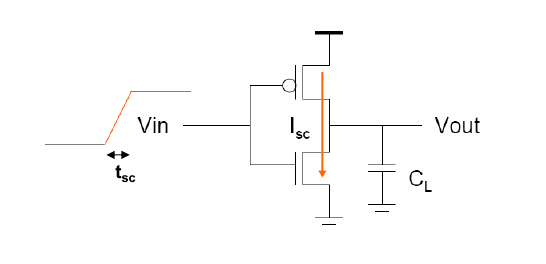
\includegraphics[width=0.7\textwidth]{images/logic_gate_1}
    \caption{Representation of a Logic Gate during a transient short-circuit: both transistors are conducting, creating a direct path to ground. $C_L$ is a parasitic capacitance responsible for most of the active energy consumption.}
    \label{fig:my_label}
\end{figure}

Active (or Dynamic) power consumption of a transition ($E_t$) is calculated by multiplying the energy necessary to switch state times the probability of this event (dependent for instance on the architecture). Power, being energy over time, equals energy times clock frequency.
\begin{align*}
E_t &= C_L \cdot V_{DD}^2 \cdot P_{0 \rightarrow 1} \\
\textrm{Power} &= C_L \cdot V_{DD}^2 \cdot P_{0 \rightarrow 1} \cdot f_{0 \rightarrow 1} = E_t \cdot \textrm{Frequency}
\end{align*}

Additionally, one needs to account for the mentioned short-circuits, absorbing a current proportional to the rising time of the signal $t_{sc}$:
\begin{align*}
E_{sc} &= t_{SC} \cdot V_{DD} \cdot I_{peak} \cdot P_{0 \rightarrow 1} \\
\textrm{Power} &= t_{sc} \cdot V_{DD} \cdot I_{peak} \cdot P_{0 \rightarrow 1} \cdot f_{0 \rightarrow 1} = E_{sc} \cdot f_{0 \rightarrow 1}
\end{align*}

Overall, dissipated power is given by the combination of:
\begin{itemize}
    \item $E_t$, mainly dependent on parasitic capacitance, therefore on number of gates and transistor size
    \item $E_{sc}$, dependent on transistor technology, size, temperature, and signal slope
    \item $E_{leakage} = V_{DD} \cdot I_{leakage}$, increasing with higher temperatures and lower threshold voltages
    \item $\textrm{Frequency}$, dependent on performance
    \item $P_{0 \rightarrow 1}$, dependent on signal statistics
\end{itemize}

Therefore:
\begin{align*}
    \textrm{Power} =&\ C_L \cdot V_{DD}^2 \cdot P_{0 \rightarrow 1} \cdot f_{0 \rightarrow 1}\\
    &\ + t_{sc} \cdot V_{DD} \cdot I_{peak} \cdot P_{0 \rightarrow 1} \cdot f_{0 \rightarrow 1}\\
    &\ + V_{DD} \cdot I_{leakage}
\end{align*}


\section{Cost Estimation}
Costs tend to generally decrease due to a number of factors. Manufacturing yield $Y$ for example, increases even without improvements in the implementation technology, adding up to an increase in production volumes which result in more amortized manufacturing costs. Costs trends also decrease because of competition effects, requiring selling prices to be close to production ones.

Experimentally, the cost $C$ of an integrated circuit is given by:
$$C=\frac{C_{die} + C_{testing} + C_{packaging}}{Y}$$
\noindent where $C_{die}$ is the cost of manufacturing a die, $C_{testing}$ that of testing a die after cutting it from a wafer, and $C_{packaging}$ that of packaging and testing the working ones. Unlike these last two costs which solely depend on the complexity of the IC, $C_{die}$ depends on more factors:
$$C_{die}=\frac{C_{wafer}}{N_{die} \cdot Y_{die}}$$
Where $N_{die}$, in turn, equals the number of dies on a round wafer of diameter $D$, minus those close to edge:
$$N_{die}=\frac{\textrm{Area of wafer}}{\textrm{Area of die}} - \textrm{Chips near the edge} = \frac{\pi \cdot \frac{1}{4} D^2}{A_{die}} - \frac{\pi \cdot D}{\sqrt{2 \cdot A_{die}}}$$
And $Y_{die}$ is given by:
$$Y_{die}=Y_{wafer} \cdot \left(1 + \frac{N_{defects} \cdot A_{die}}{\alpha}\right)^{-\alpha}$$
\noindent with $N_{defects}$ being the number of defects per unit area of the wafer, and $\alpha$ an empirical value related to manufacturing complexity.
\newline

In conclusion, it can be inferred that a designer only has control on the strong dependence that $A_{die}$ has on costs, while all other parameters only depend on the manufacturing process.


\section{Performance Evaluation}
Measuring performance is a far from trivial task. Although Moore's Law states that clock frequencies double every 15 to 18 months, architectural enhancements need to be considered as well, therefore leading to the lack of a univocal comparison criteria. An ideal metric would would be:
\begin{itemize}
    \item \textbf{Linear}: if two values differ by a certain factor, performances will also differ by the same factor.
    \item \textbf{Reliable}: a system X outperforms another system Y if the metric indicates so.
    \item \textbf{Repeatable}: measurements results are consistent across repetitions, with a given amount of uncertainty.
    \item \textbf{Easy to use}: more people will adopt the metric and the probability of obtaining incorrect results decreases.
    \item \textbf{Consistent}: units and definition are the same across different systems and configurations.
    \item \textbf{Independent}: the definition is univocal and is not affected by external influences.
\end{itemize}

\begin{example}
\textbf{Clock Frequency} \\
This metric is repeatable, easy to measure, consistent and independent, but NOT linear and reliable. For instance, it doesn't take into account the amount of computation carried out within a clock cycle, nor it considers the interaction with the I/O system.
\end{example}

\begin{example}
\textbf{Millions of Instructions Per Second (MIPS)} \\
Although repeatable, independent, and easy to measure, this metric is NOT linear, reliable, nor consistent: as for the Clock Frequency, the meaning of "instruction" and its computational load vary from architecture to architecture.
\end{example}

\begin{example}
\textbf{MOPS and MFLOPS} \\
These two metrics try to solve the inconsistency of MIPS by considering (respectively) only integer and floating-point operations, therefore defining more strictly the concept of "instruction". However, it still doesn't consider the differences in implementation of the operations, possibly resulting in misleading figures.
\end{example}

\begin{example}
\textbf{Execution Time} \\
Execution Time meets all the properties listed above. It includes both the time actually spent running (CPU time), and the time spent waiting for memory and I/O operations. CPU time, in turn, consists of \textbf{User CPU time} and \textbf{System CPU time}, where the former counts the time spent when executing the task's instructions, while the latter counts the time spent for OS calls.
\end{example}

$$CPU time = N_{CLK} \cdot T_{CLK} = CPI \cdot IC \cdot T_{CLK}$$

Where $N_{CLK}$ is the number of clock cycles, $T_CLK$ the period of a cycle, $CPI$ stands for Clock Per Instruction and describes the average duration of a single instruction, and $IC$ (Instruction Count) the number of instructions of the task.

$$ CPI = \frac{\sum_{i=1}^{n}IC_i \cdot CPI_i}{IC}$$

Where $n$ is the total number of instructions of the ISA of a certain processor, and $IC_i$ and $CPI_i$ are respectively the IC and CPI of the $i-th$ instruction.

\section{Benchmarks}
A benchmark is a suite of tasks that aims at mimicking the expected workload of a given computing system, in order to compare the performance of different systems. Benchmarks come in many types:
\begin{itemize}
    \item \textbf{Real Applications} have many problems related to portability and variability of the workload across repetitions due to the number of employed options.
    \item \textbf{Modified (Scripted) Applications} are Real Applications with improved portability thanks to, for instance, the removal or simulation of I/O operations.
    \item \textbf{Kernels} are key sections of real applications extracted to evaluate the performance of individual features.
    \item \textbf{Synthetic Benchmarks} are similar to kernels but are just simulations of instructions frequencies with no practical usefulness.
    \item \textbf{Toy Benchmarks} consist of 10 to 100 lines of code running simple and portable algorithms with known solutions.
\end{itemize}

Since companies tend to only select those which highlight the performance of their products, benchmarks are given out among suites with specific rules on compilation options and source code modifications. Depending on the target architecture, benchmarks can be of different kinds from Desktop Computing to Servers or Embedded Systems.

In order to evaluate the performance of a suite, two geometric means are used: one for integer benchmarks, and for floating-point ones. A geometric mean is calculated as:

$$ G = \sqrt[N]{\prod_{j=1}^{N}\left(\frac{T_{e_j}}{T_{R_j}}\right)} $$

With N being the number of programs, $T_{e_j}$ the execution time of the $j$-th task, and $T_{R_j}$ the reference execution time of the $j$-th program. A geometric mean offers the advantage of maintaining consistent relationships regardless of the reference machine, but long and short tasks will have the same weight, encouraging engineers to focus on easy-to improve benchmarks instead of focusing on the slowest applications. Therefore, a number of other criteria exist:

\begin{itemize}
    \item \textbf{Total Execution Time} \\
    $$ T = \sum_{j=1}^NT_{e_j}$$
    \item \textbf{Average Execution Time} \\
    $$ \overline{T}_e = \frac{1}{N} \sum_{j=1}^NT_{e_j}$$
    \item \textbf{Weighted Execution Time} \\
    $$ T_{e_w} = \sum_{j=1}^Nw_jT_{e_j}$$
    \item \textbf{Equal Time Weighing} \\
    $$ w_j = \frac{1}{T_{e_j} \cdot \sum_{j=1}^N\frac{1}{T_{e_j}}}$$
    
\end{itemize}

\section{Design of Computing Systems}
Designing a system or architecture is a multi-variable and multi-objective optimization problem, involving \textit{execution time (T)}, \textit{cost (C)}, and \textit{power consumption (P)}.

E basta, mi son rotto le balle di sto capitolo (slide 52).

